\documentclass[12pt,a4paper]{report}
\usepackage[spanish]{babel} 
\usepackage{titlesec}
\usepackage{chngcntr}
\usepackage[margin=2cm]{geometry}
\usepackage{booktabs,tabularx,longtable}
\usepackage[table]{xcolor}
\usepackage{enumitem,fancyhdr}
\usepackage{graphicx}
\usepackage{ragged2e}
\usepackage{tocloft}
\usepackage{float}
\usepackage{hyperref}

\addto\captionsspanish{\renewcommand{\contentsname}{Índice}}

% --- CONFIGURACIÓN DE FIGURAS ---
\counterwithout{figure}{chapter}
\renewcommand{\cftfigpresnum}{Figura }
\renewcommand{\cftfigaftersnum}{:}
\setlength{\cftfignumwidth}{5.5em}


% 2. Registrar la lista en tocloft para habilitar \cftdiagramapresnum
\newlistof{diagrama}{lod}{Índice de diagramas}

% 3. Aplicar el formato deseado
\renewcommand{\cftdiagramapresnum}{Diagrama }
\renewcommand{\cftdiagramaaftersnum}{:}
\setlength{\cftdiagramanumwidth}{6.5em}

% 4. Mantener la numeración continua (1, 2, 3...) sin número de capítulo
\counterwithout{diagrama}{chapter}


% Modifica el formato del comando \chapter
\titleformat{\chapter}[hang]
{\normalfont\huge\bfseries} % Estilo del texto (Grande y Negrita)
{\thechapter\ - }           % Lo que va antes del título: "1 - "
{0pt}                       % Espacio entre el número y el título
{\MakeUppercase}            % Fuerza el título a estar en MAYÚSCULAS




\definecolor{ink}{HTML}{263746}\definecolor{red}{HTML}{9A3E3E}\definecolor{pale}{HTML}{FAEEEE}
\hypersetup{colorlinks=true,linkcolor=red,urlcolor=red}
\renewcommand{\headrulewidth}{0.4pt}

% --- CONFIGURACIÓN DE FIGURAS ---
\counterwithout{figure}{chapter}
\renewcommand{\cftfigpresnum}{Figura }
\renewcommand{\cftfigaftersnum}{:}
\setlength{\cftfignumwidth}{4.5em}

% --- CONFIGURACIÓN DE DIAGRAMAS (SIN CONFLICTOS) ---
% 1. Definir el entorno flotante con el paquete 'float'
\newfloat{diagrama}{htbp}{lod}
\floatname{diagrama}{Diagrama}

% 2. Configurar su índice con 'tocloft'

\renewcommand{\cftdiagramapresnum}{Diagrama }
\renewcommand{\cftdiagramaaftersnum}{:}
\setlength{\cftdiagramanumwidth}{6em}


\begin{document}
\RaggedRight

\begin{titlepage}\centering{\color{ink}\Large\bfseries UNIVERSIDAD TECNOLÓGICA NACIONAL\par}\vspace{0.5cm}{\normalsize\bfseries INSTITUTO NACIONAL SUPERIOR DEL PROFESORADO TÉCNICO\par}

\vspace{1.6cm}\begin{figure}[h]
	\centering
	
\includegraphics[width=0.35\textwidth]{imagenes/logoUTN.png}
\end{figure}
	
\vspace{1.3cm}{\Large Informe Final\par}
\vspace{0.1cm}{\selectfont\huge\bfseries Clickfud\par}
\vspace{0.1cm}{\selectfont\huge\bfseries Sistema  de pedidos de comida a domicilio ó para llevar\par}
\vspace{1.2cm}{\Large Trabajo final de Seminario 3.603}
\vspace{1.2cm}\textit{\Large \\Imperi, Jonatan Eduardo \\151957 \\jonatan.imperi@alu.inspt.utn.edu.ar}
\vspace{1.2cm}{\Large \\Fecha de presentación \\ \textit{19/11/2026}}
\vspace{1.2cm}{\Large{\\Docente de cátedra\\Prof. Mermoz, Daniel}}
\end{titlepage}

\thispagestyle{empty} % Quita el número solo en esta página

\newpage
~
\pagenumbering{Roman} % Cambia a romanos mayúsculas
\newpage

\section*{\Huge RESUMEN}
\begin{justify}
El desarrollo de ClickFud  tiene como finalidad entregar al cliente un sistema donde recibir y gestionar pedidos de su restaurante. Los consumidores tienen acceso a la página web por medio de cualquier navegador en donde hacen los pedidos, evitando de esta manera tener la obligación de descargar una aplicación dedicada a tal fin. El sistema completo se compone de tres interfaces visuales con las que se interactúan los distintos tipo de usuario.

La interfaz principal, utilizada por el administrador del local es una aplicación web que recibe y gestiona los pedidos entrantes, tener el control de las comandas y los pagos, tener el contacto de los clientes y además poseer un chat con el cual poder comunicarse con los repartidores a domicilio.

La segunda interfaz es una aplicación móvil para Android destinada a los repartidores del local para dar aviso de los envíos pendientes, confirmar las entregas y brindarles servicio de mapa con la ruta hacia el destino de entrega como también un chat para poder comunicarse con el restaurante.

La tercera interfaz orientada al público, es una tienda virtual que muestra las platos disponibles, ofrece a opción de retirar por el local o recibir el pedido a domicilio. Elegir el medio de pago y concretar la compra.
\end{justify}
\newpage
~
\newpage

\section*{\Huge ABSTRACT}
\begin{justify}
The development of ClickFud aims to provide the client with a system for receiving and managing restaurant orders. Consumers access the website via any web browser to place orders, thereby avoiding the need to download a dedicated app. The complete system consists of three interactive visual interfaces.

The main interface, used by the establishment's administrator, is a web application that receives and manages incoming orders; it handles order tracking and payments, maintains customedr contact details, and includes a chat feature for communicating with delivery drivers.

The second interface is an Android mobile app designed for the establishment's delivery drivers; it notifies them of pending deliveries, allows them to confirm completed deliveries, provides mapping services with routes to the destination, and includes a chat function for communicating with the restaurant.

The third interface, aimed at the public, is an online store that displays available dishes and offers the choice between pickup and home delivery, allowing customers to select a payment method and complete their purchase.
\end{justify}
\newpage
~
\newpage

\tableofcontents
\newpage
\listoffigures
\newpage
\listofdiagrama % <-- Nuevo comando generado automáticamente
\newpage


\newpage
~
\newpage
\texttt{}
\chapter{Introducción}
\begin{justify}
El rubro gastronómico es de los que funcionan casi todos los días de la semana ya que la demanda de consumo lo requiere y hace posible. De esta manera, los locales que trabajan haciendo entregas a domicilio como también los que preparan el pedido para ser retirados por el cliente en el lugar, necesitan gestionar y procesar tales encargos. Hasta no hace mucho tiempo, los pedidos realizados de forma remota se hacían mediante llamadas telefónicas exclusivamente, y aunque hoy en día algunos optan por la mensajería instantánea, lo más habitual es el uso de aplicaciones que conectan el negocio de comida con miles de clientes cercanos y se encarga de la logística de entrega.
El principal problema que presentan dichas aplicaciones es el encarecimiento del producto final para el cliente como consecuencia del costo de las comisiones para los vendedores, lo cual puede inhibir el consumo.
El motivo para la creación de este sistema es reducir esos costos como también prescindir de sus métodos de venta que consisten en incentivar constantemente al consumidor con ofertas que duran muy poco tiempo.
\end{justify}

\pagenumbering{arabic}
	
\chapter{Estado del arte}
\begin{justify}
Las plataformas de delivery (pedidosYa, Rappi) ofrecen alcance y logística, pero cobran comisiones por pedido que reducen el margen del comercio. Por otro lado, los sistemas de gestión (FUDO, Bistrosoft, Kyte) resuelven la operación interna del local con un alcance funcional amplio, aunque no están orientados a un circuito de delivery propio de punta a punta. Este proyecto propone un modelo híbrido: un sistema de alcance acotado que integra en una sola solución la gestión de pedidos y cobros del local, una web de compra para clientes y una aplicación para repartidores propios, eliminando la comisión por pedido a costa de un menor número de funcionalidades.
\end{justify}

\section{PedidosYa}
\begin{justify}
Se encuentra entre las aplicaciones más conocidas de entrega a domicilio. PedidosYa no cobra una comisión fija única para todos, sino un porcentaje variable sobre el valor de cada pedido. En muchos casos arranca con promociones iniciales (por ejemplo, 5 por ciento el primer mes, 15 por ciento el segundo y un 25 por ciento a 30 por ciento a partir del tercer mes o según el tipo de contrato). Estos costos de comisión impulsan a que los locales aumenten sus precios finales en la aplicación en comparación a los precios de manera directa.
El esquema de pago hacia el negocio se hace de forma semanal
\end{justify}

\section{Rappi}
\begin{justify}
Muy parecida a PedidosYa pero con diferencias en condiciones de negocio, otro tipos de comisiones, distintos acuerdos, etc.
\end{justify}

\section{FUDO}
\begin{justify}
Fudo es una plataforma de gestión gastronómica en la nube que funciona 100 por ciento desde el navegador de una computadora, tablet o celular, sin necesidad de instalaciones complejas. Centraliza el salón, la cocina, el delivery, el control de stock, la caja y la facturación electrónica en un solo sistema.
\end{justify}
\chapter{Definición del problema}
\begin{justify}
La dependencia casi total de las empresas de delivery, con comisiones elevadas y condiciones contractuales inconvenientes son el factor principal para promover el cambio; Mientras que las comisiones dejan al comercio la disyuntiva entre trasladar los precios finales perdiendo ventas ó mantener los precios finales obteniendo menores ganancias, las condiciones inconvenientes que imponen estas aplicaciones son las de efectuar los pagos de forma semanal o quincenal reteniendo así capital que podría estar usando el negocio para sus propios gastos sin contar además que ese dinero ya le pertenece.

Otra desventaja de los sistemas en uso, es la propiedad de los datos, ya que las aplicaciones impulsan ventas, pero limitan el acceso a los mismos. Además de los productos que se venden y sus cantidades, el dato que más se pierde es el contacto directo con los clientes, si son de la zona o no. El comercio no tiene la posibilidad de analizar de forma directa a través de estas aplicaciones lo que vendió y por lo tanto si desea hacerlo, estará obligado a realizarlo por otro medio.
\end{justify}

\newpage

\section{Análisis FODA}
\begin{justify}
Para este análisis se toma como referencia la comparación realizada en el estado del arte entre plataformas de delivery y sistemas de gestión para restaurantes. Dado que el sistema se encuentra en etapa de diseño, las fortalezas y debilidades se plantean como características previstas y no como resultados medidos. A partir de este gráfico se identifican los aspectos que el proyecto debe potenciar y los riesgos que debe considerar en su desarrollo.
\end{justify}

\vspace{1cm}

\begin{figure}[htbp]
	\centering
	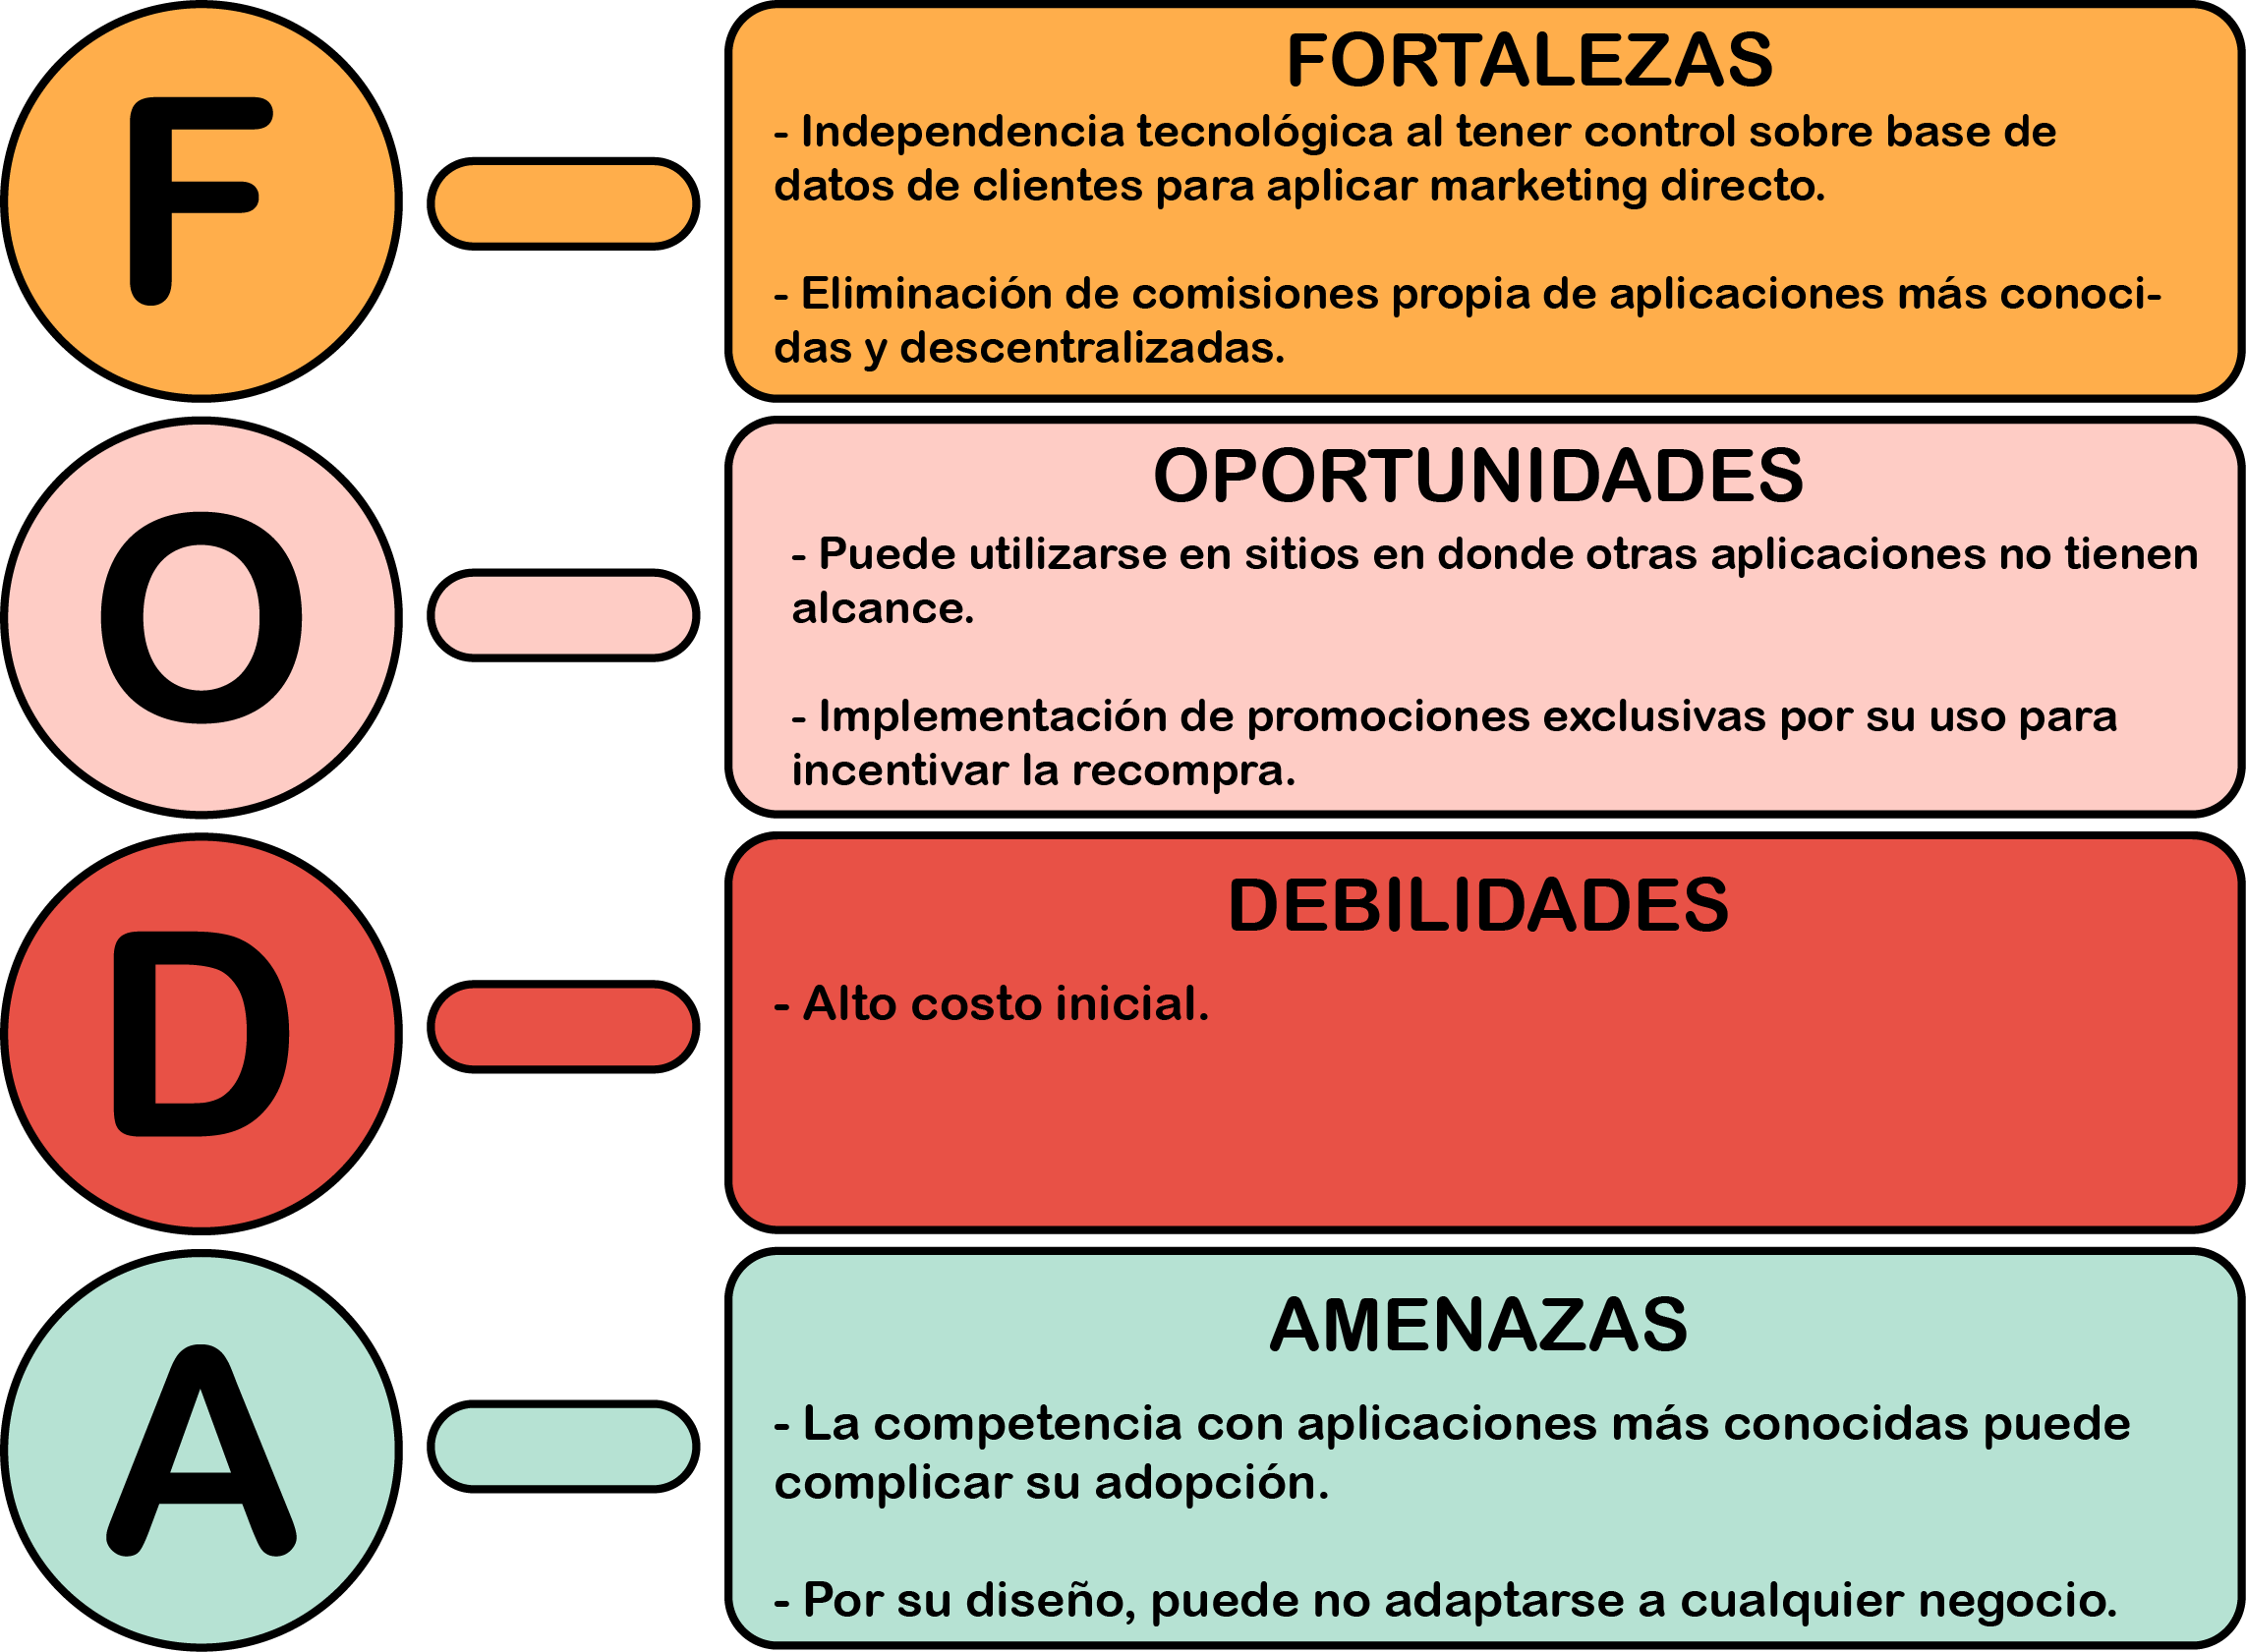
\includegraphics[width=0.90\textwidth]{imagenes/analisisFODAClickFud.png}
	\caption{Gráfico de análisis FODA}
\end{figure}
\chapter{Solución propuesta}
\begin{justify}
El sistema propuesto es una solución integral para la gestión de pedidos de restaurantes que operan su propio servicio de entrega a domicilio, sin intermediarios ni comisiones por pedido. Está dirigido a comercios gastronómicos de pequeña escala y involucra a tres tipos de usuarios: los clientes, el personal del local y los repartidores.

La solución se compone de tres módulos que operan de forma coordinada. Un módulo de compra en línea permite a los clientes consultar el menú, realizar pedidos, pagar y seguir el estado de su entrega. Un módulo de gestión para el local recibe esos pedidos en tiempo real, permite también cargar los que ingresan por mostrador o teléfono, administrar el menú, registrar cobros y asignar cada pedido a un repartidor. Por último, un módulo para repartidores les permite ver sus entregas asignadas, informar su avance y registrar el cobro cuando corresponde.

De este modo, el restaurante concentra en un único circuito la recepción, preparación, cobro y entrega de sus pedidos, y conserva la relación y los datos de sus clientes. El sistema se limita deliberadamente a las funciones esenciales del delivery propio, dejando fuera aspectos como la facturación electrónica o la gestión de inventario, con el fin de mantener una solución simple y de bajo costo.
\end{justify}
	
\newpage
\section{Análisis de requisitos}
\vspace{0.5cm}
\begin{center}
\textbf{Requerimientos funcionales}
\end{center}
\vspace{0.5cm}
\textbf{Web del cliente}
\begin{itemize}
	\item Ver el menú con categorías, precios y disponibilidad.
	\item Armar un carrito y confirmar el pedido indicando la dirección de entrega o el retiro en el local.
	\item Pagar en línea (por ejemplo con Mercado Pago) o elegir pago contra entrega.
	\item Ver el estado del pedido (recibido, en preparación, en camino, entregado).
\end{itemize}

\vspace{0.5cm}
\textbf{Aplicación de escritorio del local}
\begin{itemize}
	\item Recibir en tiempo real los pedidos de la web.
	\item Cambiar el estado de un pedido y asignarlo a un repartidor.
	\item Registrar cobros y cerrar la caja del día.
	\item Administrar el menú (altas, bajas, precios y disponibilidad).
	\item Consultar reportes básicos de ventas por día.	
\end{itemize}

\vspace{0.5cm}
\textbf{Aplicación móvil del repartidor}
\begin{itemize}
	\item Iniciar sesión y ver los pedidos asignados.
	\item Ver la dirección y los datos de entrega.
	\item Actualizar el estado de la entrega (retirado, entregado).
	\item Registrar el cobro si el pedido es contra entrega.
\end{itemize}

\vspace{0.5cm}
\begin{center}
	\textbf{Requerimientos no funcionales}
\end{center}
\vspace{0.5cm}

\begin{itemize}
	\item Seguridad: contraseñas cifradas, comunicación por HTTPS y permisos según el rol. Los datos de tarjeta no se almacenan, los procesa el proveedor de pagos.
	\item Tiempo real: el local debe ver un pedido nuevo casi de inmediato.
	\item Disponibilidad: el sistema debe estar operativo en el horario de atención del restaurante.
	\item Usabilidad: interfaces simples que no requieran capacitación larga, con la aplicación de escritorio pensada para uso rápido en horas pico.
	\item Mantenibilidad: código modular, con un backend único que compartan las tres aplicaciones.
	\item Compatibilidad: la web debe funcionar en los navegadores actuales y en pantallas de celular, y la app móvil en Android.
	\item Escalabilidad: capacidad para sumar más pedidos y repartidores sin rediseñar el sistema.	
\end{itemize}

\newpage

\section{Especificaciones del sistema}
\begin{justify}
El sistema propuesto consiste en una plataforma integrada para la gestión de pedidos de un restaurante, compuesta por tres aplicaciones que comparten un mismo servidor y una base de datos centralizada.

Los clientes accederán al sistema mediante una aplicación web, desde la cual podrán consultar el menú, personalizar sus pedidos y realizar compras sin necesidad de instalar software adicional. Esta aplicación será desarrollada utilizando React y TypeScript, permitiendo una interfaz moderna, adaptable a dispositivos móviles y de fácil mantenimiento.

El restaurante dispondrá de una aplicación de escritorio, instalada en una computadora del local, encargada de recibir y administrar los pedidos en tiempo real, gestionar el menú, controlar el estado de las órdenes y administrar la información del negocio. Esta aplicación será desarrollada en Kotlin utilizando Compose Multiplatform, obteniendo una interfaz nativa y un mejor acceso a los recursos del sistema operativo, como impresoras y archivos locales.

Los repartidores utilizarán una aplicación móvil para Android, desarrollada también en Kotlin, mediante la cual recibirán las entregas asignadas, visualizarán los datos del cliente y actualizarán el estado de cada envío. 

Todas las aplicaciones se comunicarán con un backend central, desarrollado en Kotlin utilizando Spring Boot, el cual expondrá una API REST encargada de gestionar la lógica de negocio, la autenticación de usuarios, el procesamiento de pedidos y la comunicación entre los distintos componentes del sistema. Para las actualizaciones en tiempo real, como la recepción inmediata de nuevos pedidos o los cambios
de estado de una entrega, se utilizarán conexiones mediante WebSockets.

La información del sistema será almacenada en una base de datos PostgreSQL, elegida por su confiabilidad, soporte para transacciones, integridad de los datos y capacidad de escalabilidad, características fundamentales para una aplicación comercial.

En cuanto a la seguridad, el acceso al sistema se realizará mediante autenticación basada en JSON Web Tokens (JWT), mientras que las contraseñas serán almacenadas utilizando algoritmos de hash seguros. Toda la comunicación entre las aplicaciones y el servidor se realizará mediante el protocolo HTTPS, garantizando la confidencialidad e integridad de la información transmitida.

Para el procesamiento de pagos electrónicos, el sistema se integrará con una pasarela de pagos externa, como Mercado Pago, permitiendo realizar pagos mediante transferencia, código QR o tarjeta de manera segura, sin almacenar información financiera sensible dentro del sistema.

La arquitectura propuesta permitirá mantener una única fuente de información para todas las aplicaciones, facilitando el mantenimiento, la escalabilidad y la incorporación de nuevas funcionalidades en el futuro.
\end{justify}

\newpage
\section{Análisis del sistema}
\begin{diagrama}[htbp]
	\centering
	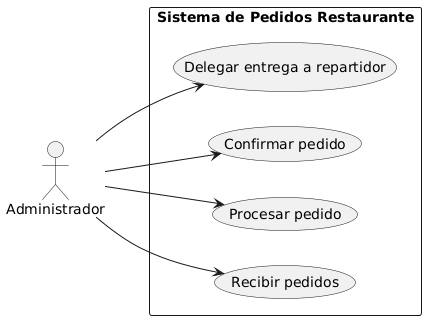
\includegraphics[width=0.8\textwidth]{diagramas/caso_uso/casoUsoAdministrador.png}
	\caption{Caso uso usuario administrador}
\end{diagrama}

\begin{diagrama}[htbp]
	\centering
	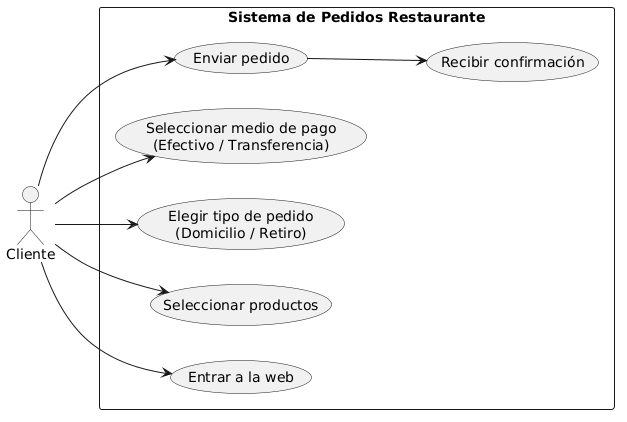
\includegraphics[width=0.8\textwidth]{diagramas/caso_uso/casoUsoCliente.png}
	\caption{Caso uso usuario cliente}
\end{diagrama}

\begin{diagrama}[htbp]
	\centering
	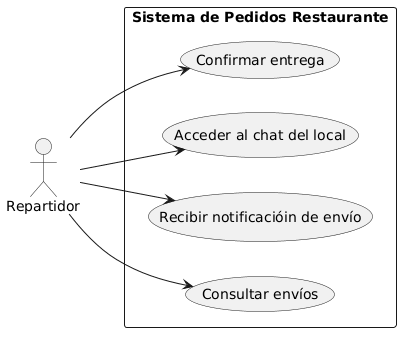
\includegraphics[width=0.8\textwidth]{diagramas/caso_uso/casoUsoRepartidor.png}
	\caption{Caso uso usuario Repartidor}
\end{diagrama}

\begin{diagrama}[htbp]
	\centering
	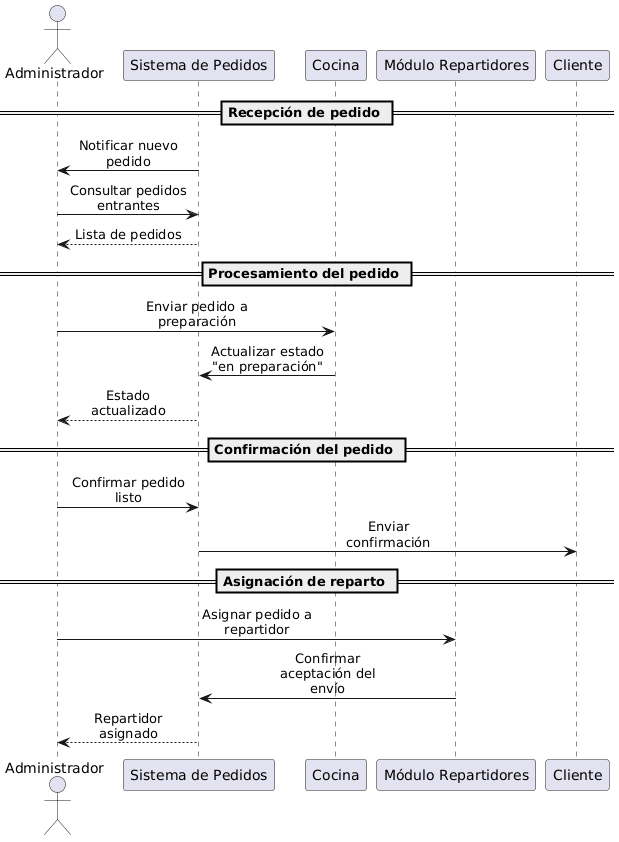
\includegraphics[width=0.8\textwidth]{diagramas/de_secuencia/diagramaSecuenciaAdministrador.png}
	\caption{De secuencia usuario administrador}
\end{diagrama}

\begin{diagrama}[htbp]
	\centering
	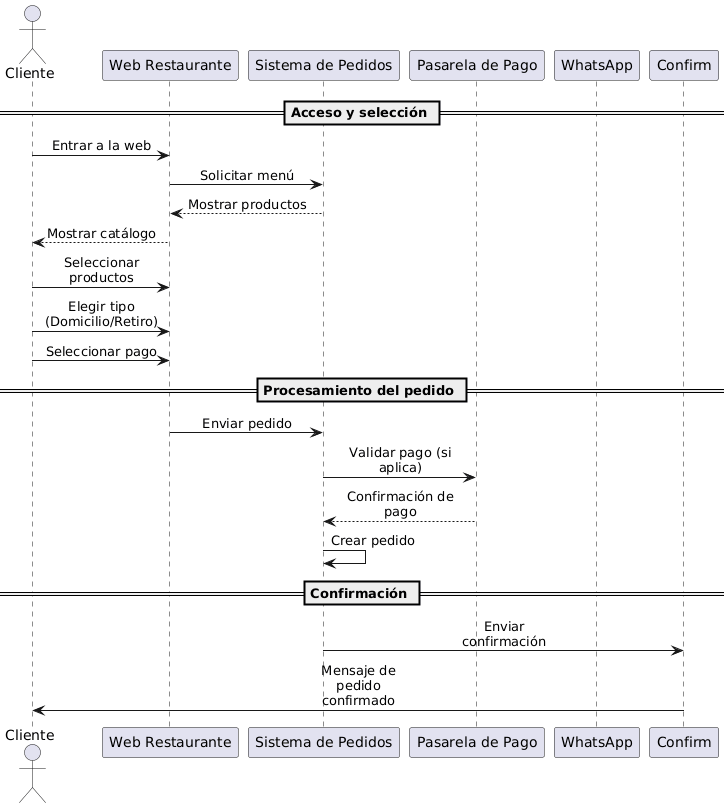
\includegraphics[width=0.8\textwidth]{diagramas/de_secuencia/diagramaSecuenciaCliente.png}
	\caption{De secuencia usuario cliente}
\end{diagrama}

\begin{diagrama}[htbp]
	\centering
	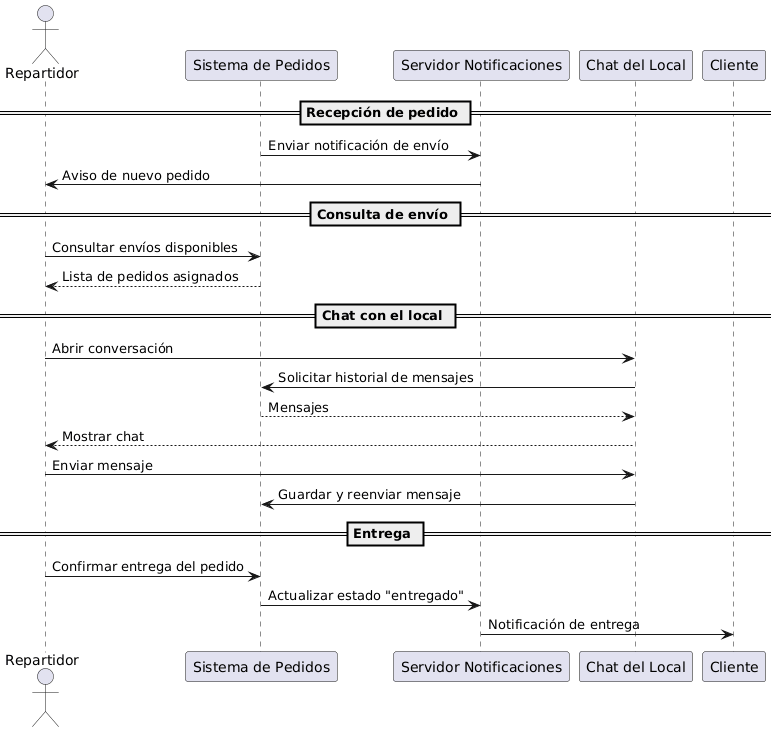
\includegraphics[width=0.8\textwidth]{diagramas/de_secuencia/diagramaSecuenciaRepartidor.png}
	\caption{De secuencia usuario repartidor}
\end{diagrama}
\chapter{Resultados}

\chapter{Conclusiones}

\section{Referencias}

\section{Bibliografía}

\section{Anexos}




\end{document}
